
\documentclass[11pt,oneside,letterpaper]{article}

% graphicx package, useful for including eps and pdf graphics
% include graphics with the command \includegraphics
\usepackage{graphicx}
\DeclareGraphicsExtensions{.pdf,.png,.jpg}

% cite package, to clean up citations in the main text. Do not remove.
\usepackage{cite}

\usepackage{color} 

\usepackage{parskip}

% Use doublespacing - comment out for single spacing
%\usepackage{setspace} 
%\doublespacing

% Text layout
\usepackage{geometry}
\geometry{textwidth=15.25cm} % 16cm for PLoS
\geometry{textheight=22cm}

% Bold the 'Figure #' in the caption and separate it with a period
% Captions will be left justified
%\usepackage[labelfont=bf,labelsep=period,font=doublespacing]{caption}
\usepackage[labelfont=bf,labelsep=period,font=small]{caption}

\usepackage{float}

% Use the PLoS provided bibtex style
\bibliographystyle{plos2009}

% Remove brackets from numbering in List of References
\makeatletter
\renewcommand{\@biblabel}[1]{\quad#1.}
\makeatother

\usepackage{authblk}
\renewcommand\Authands{ \& }

% comments
\usepackage{ulem}
\definecolor{purple}{rgb}{0.459,0.109,0.538}
\def\tb#1#2{\sout{#1} \textcolor{purple}{#2}} 
\def\tbc#1{\textcolor{purple}{[#1]}}
\definecolor{blue}{rgb}{0.324,0.609,0.708}
\def\ar#1#2{\sout{#1} \textcolor{blue}{#2}} 
\def\arc#1{\textcolor{blue}{[#1]}}
\definecolor{green}{rgb}{0.513,0.73,0.442} 
\def\mp#1#2{\sout{#1} \textcolor{green}{#2}} 
\def\mpc#1{\textcolor{green}{[#1]}}

\title{Canalization of the evolutionary trajectory of the human influenza virus}
\author[1,2,*]{Trevor Bedford}
\author[3,4]{Andrew Rambaut}
\author[1,2]{Mercedes Pascual}
\affil[1]{Department of Ecology and Evolutionary Biology, University of Michigan, Ann Arbor, MI, USA.}
\affil[2]{Howard Hughes Medical Institute, University of Michigan, Ann Arbor, MI, USA.}
\affil[3]{Institute of Evolutionary Biology, University of Edinburgh, Edinburgh, UK.}
\affil[4]{Fogarty International Center, National Institutes of Health, Bethesda, MD, USA.}
\affil[*]{To whom correspondence should be addressed. E-mail: bedfordt@umich.edu}
\date{\today}
 
\def\ci#1#2#3{\normalsize{\(#2\)} \scriptsize{(\(#1\), \(#3\))}} 
 
\begin{document}

%%% TITLE %%%
\maketitle


\begin{enumerate}
	\item Reconciling strong selective pressure to escape human immunity with the observed single antigenic trajectory of influenza.
	\item Difficulties of modeling influenza dynamics.
	\item Simple model to account for epidemiological, genealogical, antigenic and spatial patterns.
	\item Description and justification of model.
	\item Antigenic dynamics, single path, splitting discouraged.  Clustering. Punctuated evolution.  Zig-zag movement.
	\item Relation to epidemiology patterns.  Severe and mild seasons.  Refractory years.
	\item Relation to genealogical patterns.  Spindly tree.  Low diversity.  Side branches driven extinct by antigenic innovation.
	\item Relation to spatial patterns.  Symmetric contact patterns, but asymmetric migration patterns.
	\item Shrinking mutation rate to approximate influenza H1N1 / B.
	\item Model supports the use of antigenic cartography.  Interdependence of genealogical and antigenic patterns.
	\item Model works well in higher dimensions.  Further supporting a 1d antigenic reality.
	\item Prediction.  General patterns of antigenic flux.
	\item Preemptively distinguishing trunk from side branches.  Mutational spectrum.  Antigenic flux.  Spatial origin of mutations of large effect.  Refractory evolution.
	\item Canalization of influenza's evolutionary trajectory.
\end{enumerate}

\begin{abstract}
Influenza A (H3N2) has persisted in the human population since 1968 through continued seasonal epidemics.  During this time, influenza underwent substantial antigenic drift, allowing it infect a large fraction of the human population year after year.  Understanding the process of antigenic evolution is key to our efforts of disease control and surveillance, i.e. the emergence of new antigenic variants require corresponding updates of the influenza vaccine.  Influenza's antigenic evolution over this time period has been experimentally characterized, resulting in an two-dimensional `antigenic map' detailing antigenic similarity between strains.  The genetic relationships among strains from 1968 to 2007 have also been distinguished, showing a characteristic ladder-like genealogical tree.  This work seeks to simultaneously model the antigenic patterns and the genealogical patterns exhibited by the influenza virus.  Here, we use a large-scale individual-based model to show that evolution in a Euclidean antigenic space results a close correspondence between model behavior and available data in terms of antigenic map and in terms of genealogical tree.  This model is also used to investigate patterns of spatial movement of between northern, southern and tropical regions.
\end{abstract}

\section*{Introduction}

Epidemic influenza is responsible for between 250,000 and 500,000 global deaths annually, with influenza A (H3N2) having historically caused the bulk of human mortality and morbidity \cite{flufactsheet}.  Influenza A (H3N2) has continually circulated within the human population since its introduction in 1968, exhibiting recurrent seasonal epidemics in temperate regions and less periodic transmission in the tropics.  Annual winter epidemics of H3N2 influenza show average cumulative attack rates of 3--8\% \cite{Monto93,Koelle09}.  Since its emergence, influenza A H3N2 has continually evolved both genetically and antigenically.  Without antigenic drift, influenza would be confined to childhood infections and show lower overall incidence.  Phylogenetic analysis of the genetic evolution of influenza H3N2 has revealed a distinctive genealogical tree showing a single predominant trunk lineage and side branches that persist for only 1--5 years before going extinct \cite{Fitch97}.  This tree shape is indicative of serial replacement of strains over time; H3N2 influenza shows rapid evolution, but low standing genetic diversity.

This observation has remained puzzling from an epidemiological standpoint.  Antigenic evolution occurs rapidly; in this case, why doesn't one lineage of influenza move in one antigenic direction and another lineage in a tangential antigenic direction?  Strong diversifying selection exists to escape from human immunity, why then do we see serial replacement of strains rather than continual accumulation of antigenic and genetic diversity?  Indeed simple epidemiological models show explosive diversity of genotype and phenotype over time \cite{Ferguson03,Tria05}.  Previous work has sought model-based explanations of the limited diversity of influenza, relying on short-lived strain-transcending immunity \cite{Ferguson03,Tria05}, complex genotype-to-phenotype maps \cite{Koelle06} or a limited repertoire of antigenic phenotypes \cite{Recker07}. 

Fortunately, influenza permits experimental characterization of antigenic phenotype.  Through the hemagglutination inhibition (HI) assay, the cross-reactivity of antisera and antigen pairs from different virus strains may be compared \cite{Hirst43}.  Through the use of dimensionality reduction techniques, panels of HI comparisons can yield two-dimensional antigenic maps, representing antigenic similarity and distance as an easily visualized and quantified measure \cite{Smith04}.  The antigenic path traced by influenza A (H3N2) from 1968 until present is largely linearly, showing serial replacement of one strain by another; there are no major bifurcations of antigenic phenotype \cite{Smith04}.  Thus the genetic and antigenic patterns of H3N2 influenza appear consistent; both antigenic map and genealogical tree lack branching events wherein separate lineages of influenza move in different antigenic/genetic directions.

Herein, we seek to further reconcile antigenic and genetic patterns of influenza evolution using a large-scale individual-based model.  Our approach seeks to simultaneously and directly model the antigenic map and genealogical tree of the global influenza population.  Additionally, our model incorporates geographic population structure, elucidating broad patterns of migration between regions with contrasting seasonal dynamics.

\section*{Results and Discussion}

\subsection*{A geometric model of antigenic evolution}

Using a dimensionality reduction approach, Smith and colleagues \cite{Smith04} show that a two-dimensional map adequately explains observed antigenic distances between strains.  Our model begins with this basic finding.  Here, in an analogous fashion, virus strains possess a antigenic phenotypes, which are represented geometrically as points on a plane.  After a host recovers from an infection, the phenotype of the infecting virus is added to that host's immune history.  Over time a host builds-up a repertoire of phenotypes to which it can mount an immune response.  After exposure to a virus, a host's risk of infection is proportional to the Euclidean distance between the infecting phenotype and the closest phenotype in the host's immune history.  Thus, strains possessing antigenically novel phenotypes will have a transmission advantage compared to strains whose phenotypes are more similar to phenotypes present in host immune histories.

As time goes on, strains mutate in antigenic phenotype.  Mutations are random in effect, moving a strain in a random radial direction and for an exponentially distributed distance.  Thus, most mutations have little effect on antigenic phenotype, while occasionally mutations may have large effects.  In effect, this is similar to the neutral networks implemented by Koelle et al. \cite{Koelle06}, wherein a minority of amino acid changes result in a large decrease in cross-immunity between strains.

We implemented this geometrical model in a large-scale individual-based simulation intended to describe global patterns of influenza epidemiology and evolution (for details see \textsl{Methods}).  The simulation includes multiple host populations with different seasonal forcings, hosts that contain complete immune histories of infection, and viruses that contain antigenic phenotypes.  As the simulation proceeds, infections are tracked and a genealogy connecting virus samples is constructed.  This avoids the messy intermediate step of phylogenetic inference common to phylodynamic simulations.  Results shown here are for a single simulation of 40 years of virus evolution in a population of 90 million hosts.  

\subsection*{Antigenic and epidemiological dynamics}

The virus persists over the course of the 40-year simulation, infecting a significant fraction of the host population through annual winter epidemics in temperate regions and through less periodic epidemics in the tropics (Fig.~\ref{incmap}A).  During the height of most temperate epidemics, we observe attack rates of 200 to 400 infections per 100,000 hosts per week, although some years show peak attack rates of over 1000 infections per 100,000 hosts per week.  Across replicate simulations, we observe average yearly attack rates of 3.4\% in the temperate regions and rates of 3.8\% in the tropics.  Yearly attack rates show significant variation, with a 95\% range across replicates of 0\% to 13\% in temperate regions and 0\% to 12\% in the tropics.  Under these parameter values, but without antigenic evolution, we would expect yearly attack rates of 1.1\%.

Over the course of the simulation, the virus population evolves in antigenic phenotype (Fig.~\ref{incmap}B).  Here, there are a number of distinct antigenic phenotypes found over the course of the simulation (Fig.~\ref{phenotypes}A).  Mutations move virus phenotypes in antigenic space and the resulting novel phenotypes outcompete older `spent' virus phenotypes.  There are a handful of highly abundant phenotypes sampled repeatedly and a large number of phenotypes appearing a low abundance (Fig.~\ref{phenotypes}A).  These low abundance phenotypes form clouds around the high abundance phenotypes from which they arise.  The appearance of the clusters in the antigenic map (Fig.~\ref{incmap}B) come from the regular spacing of high abundance phenotypes (Fig.~\ref{phenotypes}A) combined with experimental measurement noise (see \textsl{Methods}).

Remarkably, although antigenic phenotype is free to mutate in any direction in the two-dimensional space, selection pressures force the virus population to move in a straight-line in antigenic phenotype (Fig.~\ref{phenotypes}A).  Across replicate simulations, 93\% (interquartile range 91--98\%) of the variance of antigenic phenotype can be explained by a single dimension of variation.  This mirrors the empirical results showing a largely linear antigenic map for H3N2 influenza isolates from 1968 to 2003 \cite{Smith04}.  Because of the largely one-dimensional movement, antigenic distance from the original phenotype increases in a linear fashion with time (Fig.~\ref{phenotypes}B).  Significant two-dimensional drift would be seen as a less than linear increase of antigenic distance with time.  It's apparent here that antigenic evolution occurs in a punctuated fashion; periods of relative stasis are interspersed with rapid antigenic change.  Furthermore, large discontinuities in antigenic phenotype frequently correspond to cluster transition events.  Over the entire 40-year simulation, antigenic drift moves the virus population at an average rate across replicates of 0.88 antigenic units per year (interquartile range 0.78--0.99).  Looking at a finer scale gives a similar picture; across replicates year-to-year antigenic drift is 1.30 antigenic units (interquartile range 0.38--1.65), measured as the distance from the centroid of phenotypes in year $t$ to the centroid of phenotypes in year $t+1$.

Antigenic and epidemiological dynamics show a fundamental linkage, wherein large jumps of antigenic phenotype result in increased rates of infection (Fig.~\ref{incmap}A and B).  We observe a general correlation between year-to-year antigenic drift and attack rates the following year (corr = 0.28, Fig.~\ref{driftvsinc}A).  Similar patterns have been noted in influenza H3N2 in correlating excess mortality and antigenic evolution \cite{Wu10}.  Additionally, as noted by Koelle et al.\cite{Koelle06}, we commonly observe refractory years after a year of severe incidence brought about by antigenic drift (Fig.~\ref{incmap}A).  In general, years with low attack rates follow both unusually severe and unusually light years (Fig.~\ref{driftvsinc}B).

\subsection*{Evolutionary dynamics}

The genealogical tree connecting the evolving virus population appears characteristically sparse with pronounced trunk and short side branches  (Fig.~\ref{genealogy}).  This tree shape is reflected in low levels of genealogical diversity measured at 5.68 years.  This means that 5.68 years of evolution separate two randomly sampled viruses from the population.  This low level of diversity matches what is observed in phylogenies of influenza A (H3N2) \cite{Rambaut08}.  It's apparent from the genealogy that diversity commonly increases during periods of relative evolutionary stasis (when the population remains within an antigenic cluster) and contracts during periods of antigenic drift (during cluster transition events).  A spindly genealogical tree is indicative of population turnover.  In this case, antigenic phenotypes continually mutate resulting in novel phenotypes that are more successful at spreading through the host population.  These novel phenotypes replace more primitive `spent' phenotypes, purging their genealogical diversity.  In this system, strong selective pressure exists to evolve antigenic phenotype away from human immunity.

Selective pressures can be examined by comparing which mutations are successful, i.e.\ incorporated into the progenitor trunk lineage, and which mutations fail, i.e.\ incorporated in side branches bound for extinction.  This approach has shown that, in influenza A (H3N2), epitope sites of the HA1 protein evolve faster on the trunk, while non-epitope sites of HA1 evolve faster on side branches \cite{Bush99MBE,Wolf06,Bhatt11}.  This result indicates that lineages which receive mutations to epitope sites are more likely to become progenitor (trunk) lineages, while lineages which receive mutations to non-epitope sites are more likely to more side branches.  Hence, positive selection exists on epitope mutations and purifying selection exists on non-epitope mutations.  In the present case, we compare rates and effects of mutations on trunk branches to rates and effects on side branches (Table~\ref{mktable}).  We find evidence for pervasive positive selection for antigenic change.  Trunk lineages show increased rates of phenotypic mutations (8.87$\times$), increased effect size of mutations that do occur (2.95$\times$) and, in combination, much increased rates of antigenic drift (26.11$\times$).  Additionally, trunk mutations tend to push antigenic phenotype forward along the line of primary antigenic variation (Fig.~\ref{mutspectrum}).  

Thus, lineages harboring mutations that push antigenic phenotype forward are likely to become progenitor lineages, and may be identified prospectively.  This insight forms a large part of the basis of the World Health Organization vaccine strain selection program \cite{Barr10}.  We find a roughly linear relationship between the antigenic effect of a mutation and likelihood of this mutation becoming incorporated into the trunk (Fig.~\ref{probtrunk}).

\subsection*{Spatial dynamics}

The sampled genealogy also contains detailed information on the history of migration between regions.  We find that, consistent with empirical estimates \cite{Russell08,Bedford10}, the trunk resides primarily within the tropics, where seasonal dynamics are less prevalent (Fig.~\ref{spatial}A).  Across replicate simulations, we observe that 80\% of the trunk's history is in the tropics, 10\% is in the north and 10\% is in the south.  Because host contact rates between regions are symmetrical, without seasonal forcing, we would expect equilibrium densities of one third in each region.  This result is consistent with the observed strong seasonal dynamics (Fig.~\ref{incmap}A); temperate epidemics are bound for regional extinction at the end of the winter season.  In order for a lineage to be part of the trunk and pass through a temperate region, a migration event into the temperate region at the beginning of the season and a subsequent migration event out of the temperate region before the end of the season is required.  The likelihood of this occurring depends on the rate of contact between hosts in different regions.  As rates of contact go up, the proportion of the trunk in temperate regions increases accordingly \tbc{Make figure or table}.

However, it's apparent from the genealogy that migration events between temperate regions and, to a lesser extent, from temperate regions into the tropics are relatively common (Fig.~\ref{spatial}A).  Thus, it appears that all combinations of migration events occur, but migration events out of the tropics result in evolutionary dead ends.  We calculated rates of migration based on event counts and branch length opportunity across replicate simulations.  We observe a higher average rate of migration on side branches (0.54 migs per year) compared the average rate on trunk branches (0.42 migs per year), consistent with the average migration event being deleterious to the evolutionary fate of a lineage.  Additionally, we calculated region-specific rates of migration on side branches (Fig.~\ref{spatial}B) and on trunk branches (Fig.~\ref{spatial}C).  We find that migration patterns on side branches are close to symmetric, with fairly equal rates between all regions (Fig.~\ref{spatial}B).  Extrapolating from these migration rates, we would expect a stationary distribution of 39\% north, 39\% south and 22\% tropics.  It appears that upon leaving the trunk, lineages have a slight preference to move to temperate regions.  However, migration patterns on trunk branches are highly asymmetric, with high rates of movement between temperate regions and from temperate regions into the tropics; trunk lineages rarely leave the tropics once they arrive there (Fig.~\ref{spatial}C).  Extrapolating from these rates, we arrive at an expected stationary distribution of 85\% tropics and 15\% temperate regions, in line with the observed proportion of trunk residing in the tropics.

It may at first seem counter-intuitive to see higher rates of movement from the temperate regions into the tropics along trunk branches, but it makes sense when thought of in terms of conditional probability.  Only those lineages that migrate into the tropics or those lineages which rapidly migrate between the north and south have a chance at becoming the trunk lineage, while lineage that remain within the temperate regions are doomed to extinction.  These results suggest a possible resolution to the apparent discrepancy of analyses of the global migration patterns of influenza.  Russell et al.\ \cite{Russell08} emphasize a source-sink model of movement the HA protein of influenza A (H3N2) based on their finding of a trunk lineage residing within China and the Southeast Asian tropics.  Whereas, Bedford et al.\ \cite{Bedford10} emphasize more of a global metapopulation model based on phylogenetic inference of migration rates across the entire tree.  We find that both scenarios are simultaneously possible; side branches may be highly volatile moving rapidly and symmetrically between regions, while the trunk lineage may be more stable remaining within a region (or within a highly connected network of regions) that has more persistent transmission.  In light of these results, we suggest that future work on phylogenetic models of migration take into account trunk vs.\ side branch differences in migration patterns.

\subsection*{Canalization of evolutionary trajectory}

\section*{Conclusions}

\section*{Methods}

\subsection*{Transmission model}

To characterize the joint epidemiological, genealogical, antigenic and spatial patterns of influenza, we implemented a large-scale individual-based model.  Hosts in this model are divided between three regions: North, South and Tropics.  Here, there are 30 million hosts within each of the three regions, giving $N = 9 \times 10^{7}$ hosts.  Host population size remains fixed at this number, but vital dynamics cause births and deaths of hosts at a rate of $1 / 30$ years $= 9.1 \times 10^{-5}$ per host per day.  Within each region, transmission proceeds through mass-action with contacts between hosts occurring at an average rate of $\beta = 0.3$ per host per day.  Transmission between region $i$ and region $j$ occurs at rate $r\,\beta_i$, where $r=0.001$ and is the same between each pair of regions.  Regional transmission rates in temperate regions vary according to sinusoidal seasonal forcing with amplitude $\epsilon = 0.15$ and opposite phase in the North and in the South.  Transmission rate does not vary over time in the Tropics.  Hosts recover from infection at rate $\nu = 0.2$ per host per day, giving $R_0$ in a naive host population of 1.5.  There is no super-infection in the model.

Each virus possesses an antigenic phenotype, represented as a location in Euclidean space.  Here, we primarily use a 2d antigenic location.  After recovery, a host `remembers' the phenotype of its infecting virus as part of its immune history.  When an exposure event occurs and a virus attempts to infect a host, the Euclidean distance from infecting phenotype $\phi_v$ is calculated to each of the phenotypes in the host immune history $\phi_{h_1}, \dots, \phi_{h_n}$.  Here, one unit of antigenic distance is designed to correspond to a twofold dilution of antiserum in a hemagglutination inhibition (HI) assay \cite{Smith04}. The probability that infection occurs after exposure is proportional to the distance $d$ to the closest phenotype in the host immune history.  This is $\rho = \textrm{max}\{d\,s,1\}$, where $s=0.07$ follows from experimental work on equine influenza \cite{Park09} and from studies of vaccine effectiveness \cite{Gupta06}.  Cross-immunity $\sigma$ equals $1-\rho$.

Over time viruses evolve in antigenic phenotype.  Each day there is a chance $\mu$ that an infection mutates to a new phenotype.  This mutation rate represents a phenotypic rate, rather than genetic mutation rate, and can be thought of as arising from multiple genetic sources.  Assuming 14 amino acid sites, each mutating at a rate of $10^{-5}$ gives a phenotypic mutation rate $\mu = 1.4 \times 10^{-4}$ per infection per day.  When a mutation occurs, the virus's phenotype is moved in a completely random direction $\sim \textrm{Uniform}(0,360)$ degrees.  Most mutations move phenotype a small distance, while some mutations move phenotype a larger distance $\sim \textrm{Exponential}(m)$, where $m = 0.55$ antigenic units.

\subsection*{Model output}

Daily incidence and prevalence are recorded for each region.  In this model, viruses lack sequences and so phylogenetic inference of the evolutionary relationships among strains is impossible.  Instead, we track the full genealogical tree of the virus population as the simulation proceeds.  This tree consists of an accounting of all transmission events connecting infections during the simulation.  Over the course of the simulation, samples are taken from the evolving virus population.  These samples give virus phenotypes at time of infection, but also the genealogical history connecting these samples and the phenotypes of all ancestral viruses.

\subsection*{Antigenic map}

Antigenic phenotypes are modeled as discrete entities on the Euclidean plane; multiple samples show the exact same antigenic location.  However, in empirical antigenic map of influenza A (H3N2), each strain appears in a unique location \cite{Smith04}.  We would argue that some of this pattern comes from experimental noise.  Indeed Smith et al. \cite{Smith04} find the distance between predicted measurements and observed measurements of antigen/antiserum pairs is on average 0.83 antigenic units with a standard deviation of 0.67 antigenic units.  We take this as a proxy for experimental noise and add jitter to each sampled antigenic phenotype by moving it in a random direction for an exponentially distributed distance with mean of 0.53 antigenic units.  If two samples with the same underlying antigenic phenotype are jittered in this fashion, the distance between them averages 0.83 antigenic units with a standard deviation of 0.64 units.

We added noise to each of the 5943 sampled viruses in this fashion resulting in an approximated antigenic map (Fig.~\ref{incmap}B).  Virus samples were then clustering following standard clustering algorithms.  We tried clustering by the $k$-means algorithm and also agglomerative hierarchical clustering with a variety of linkage criteron.  We found that clustering by Ward's criterion consistently outperformed other methods, when measured in terms of within-cluster and between-cluster variances.  However, the exact clustering algorithm had little effect on our overall results.

%%% REFERENCES %%%
\bibliography{/Users/bedfordt/Documents/bedford}

\pagebreak

%%% FIGURES %%%
\section*{Figures}

%%% Figure 1: incmap %%%
\begin{figure}[H]
	\centering
	\includegraphics{figures/incmap}
	\caption{\textbf{Simulation results showing epidemiological, antigenic and genealogical dynamics}. (A) Weekly timeseries of incidence of viral infection in north, south and tropics regions. (B) Antigenic map depicting phenotypes of 5943 viruses sampled over the course of the simulation, rotated so that earliest samples are on the far left and latest samples are on the far right.  To construct the map, noise was added to each sample and the resulting observations grouped into 10 clusters and colored accordingly.  Grid lines show single units of antigenic distance. (C) Genealogical tree depicting the infection history of 376 samples from the virus population.  Parent/offspring relationships were tracked over the course of the simulation, giving a direct observation of the genealogy rather than a phylogenetic inference. Cluster assignments were used to color panels (A), (B) and (C) in a consistent fashion.}
	\label{incmap}
\end{figure}

\pagebreak

%%% Figure 2: phenotypes %%%
\begin{figure}[H]
	\centering
	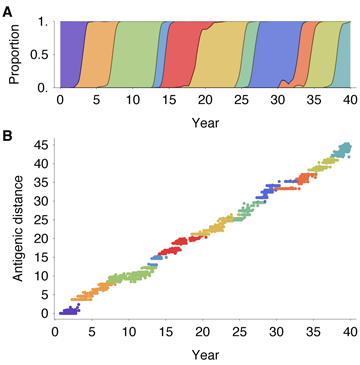
\includegraphics{figures/phenotypes}
	\caption{\textbf{Antigenic evolution over the course of the 40-year simulation}. (A) Two-dimensional antigenic phenotypes of 5943 viruses.  The figure has been rotated so that the earliest viruses are on the far left of figure and latest viruses are on the far right of the figure.  Each discrete virus phenotype is shown as a bubble, with bubble area proportional to the number of times this phenotype was sampled. (B) Antigenic distance from initial phenotype for each of 5943 virus samples relative to time of virus sampling. In both (A) and (B) viruses were sampled at a constant rate proportional to prevalence and coloring was determined by clustering of samples on the antigenic map in figure \ref{incmap}B.}
	\label{phenotypes}
\end{figure}

%%% Figure 3: genealogy %%%
\begin{figure}[H]
	\centering
	\includegraphics{figures/genealogy}
	\caption{\textbf{Evolutionary tree showing the genealogical and antigenic relationships among virus samples}.}
	\label{genealogy}
\end{figure}

%%% Figure 4: spatial %%%
\begin{figure}[H]
	\centering
	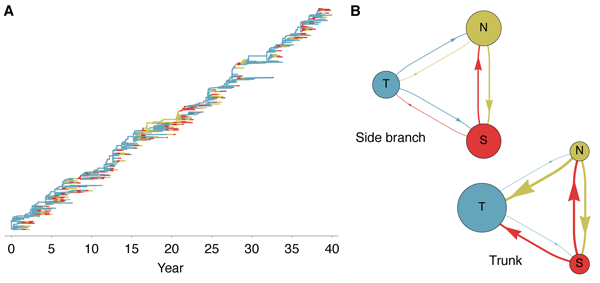
\includegraphics{figures/spatial}
	\caption{\textbf{Patterns of spatial movement of virus lineages}. (A) Evolutionary relationships among 367 viruses sampled evenly through time colored by spatial location. Lineages resides in the north, south and tropics are colored yellow, red and blue respectively. (B) Migration rates between regions on side branch lineages, and (C) Migration rates between regions on trunk lineages. Arrows denote movement of lineages and arrow width is proportional to migration rate. Circle area is proportional to the expected stationary frequency of a region given the observed migration rates.  In both cases, migration rates are calculated across 87 replicate simulations.}
	\label{spatial}
\end{figure}

%%% Figure 5: immunity %%%
\begin{figure}[H]
	\centering
	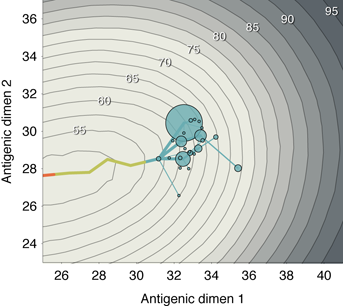
\includegraphics{figures/immunity}
	\caption{\textbf{Host immunity and antigenic history of the virus population}.  Contour lines represent the state of host immunity at the end of the 40-year simulation.  They show the mean risk of infection after a random host in the population encounters a virus bearing a particular antigenic phenotype.  Contour lines are spaced in intervals of 2.5\%. Bubbles represent antigenic phenotypes present at the end of the 40-year simulation.  The area of each bubble is proportional to the number of viruses present with this phenotype.  Lines leading into these bubbles show past antigenic history.  The current phenotypes rapidly coalesce to a trunk phenotype.  The movement of the virus population from bottom left to upper right of the figure can be seen from the antigenic history of the trunk of the virus genealogy. Shifts between antigenic clusters can also be seen as color transitions along the trunk lineage.}
	\label{immunity}
\end{figure}

%%% TABLES %%%
\section*{Tables}

%%% Figure 1: mktable %%%

\begin{table}[H]
	\centering
	\caption{\textbf{Rates of mutation and phenotypic change on trunk and side branches and mutational expectation.}}
	\label{mktable}
	\begin{tabular}{ l c c c c } 
	\hline
		 								& Baseline 	& Side branch 	& Trunk		& Trunk / side branch \\
	\hline				
	Mutation size (AG units)			& 0.55		& 0.68			& 2.02		& 2.95$\times$ \\
	Mutation rate (mut per year)		& 0.05		& 0.06			& 0.54		& 8.87$\times$ \\	
	Antigenic flux (AG units per year)	& 0.03		& 0.04			& 1.09		& 26.11$\times$ \\		
	\hline
	\end{tabular}
\end{table}

\pagebreak

%%% SUPPORTING INFORMATION %%%
\section*{Supporting Information}

\setcounter{figure}{0}
\setcounter{table}{0}
\setcounter{page}{1}
\renewcommand{\thefigure}{S\arabic{figure}}
\renewcommand{\thetable}{S\arabic{table}}
\renewcommand{\thepage}{S\arabic{page}}

%%% Figure S1: incdrift %%%
\begin{figure}[H]
	\centering
	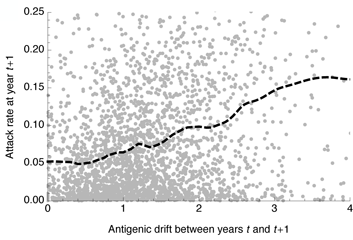
\includegraphics{figures/driftvsinc}
	\caption{\textbf{Correlation between antigenic drift and incidence and autocorrelation of attack rate}. (A) Antigenic drift measured as the distance between the centroid of phenotypes at year $t$ and the centroid of phenotypes at year $t+1$ vs.\ incidence measured as the number of samples out of $\sim6000$ in each replicate simulation taken at year $t+1$. (B) Temperate attack rate at year $t$ vs.\ temperate attack rate at year $t+1$. In both cases, individual pairs of measurements are shown as gray points and a locally-linear regression (LOESS) as black dashed line.}
	\label{driftvsinc}
\end{figure}

%%% Figure S2: mutspectrum %%%
\begin{figure}[H]
	\centering
	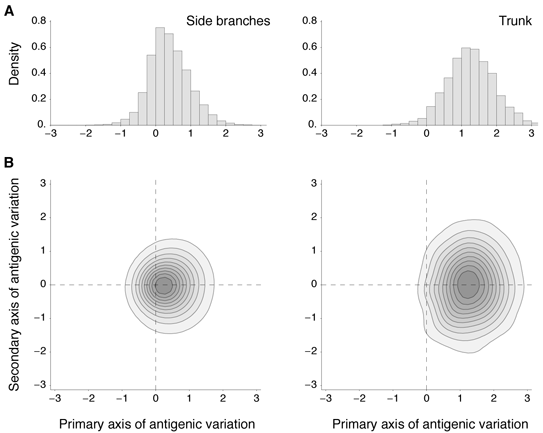
\includegraphics{figures/mutspectrum}
	\caption{\textbf{Mutation spectrum in two-dimensional antigenic space of side branch mutations and trunk mutations}. (A) Smoothed histogram of mutation effects along the axis of primary antigenic variation across 87 replicate simulations.  Left panel shows the distribution of effects of side branch mutations and the right panel shows the distribution of effects of trunk mutations. (B) Smoothed two-dimensional histogram of mutation effects along the primary and secondary axes of antigenic variation across 87 replicate simulations.  Histograms were constructed from 21,405 side branch mutations and 1584 trunk mutations.}
	\label{mutspectrum}
\end{figure}

%%% Figure S3: probtrunk %%%
\begin{figure}[H]
	\centering
	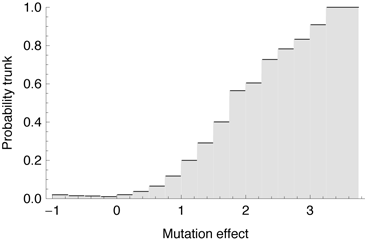
\includegraphics{figures/probtrunk}
	\caption{\textbf{Relationship between a mutation's phenotypic effect and its likelihood of being part of the trunk}. The $x$-axis represents the effect of a mutation along the line of primary antigenic variation, and the $y$-axis represents the probability that the mutation is part of the trunk.  Mutations of large effect are increasingly rare, but when they do occur are increasingly likely to be part of the trunk.}
	\label{probtrunk}
\end{figure}

\end{document}  